\chapter{Validação de Novas Abstrações de Processos}
\label{cap:validacoes}

O Capítulo \ref{cap:trabalhos-analisados} mostrou algumas pesquisas que buscam
estender a abstração de processos atual. Apesar dos vários trabalhos
demonstrarem algum tipo de benefício, muitos deles ignoram outros aspectos das
suas propostas. Por exemplo, uma abordagem que visa isolar dados para evitar
vazamento de informações faz testes que buscam por esses tipos de falhas, mas
esquecem de validar se a alteração é viável em um contexto global com uma
demanda realista.  Adicionalmente, alguns desses trabalhos baseiam-se
fortemente em \textit{microbenchmarks} o que podem evidenciar um resultado
desejado e não explicitar um efeito colateral da alteração. Em busca de
encontrar propostas de abstrações que podem ser levada para os SO atuais e
também beneficiar aplicações no espaço do usuário, levantamos e respondemos as
seguintes perguntas:

\begin{quote}
 \item \textit{RQ3:.} "Quais aplicações podem ser utilizadas para avaliar as nova abstração adicionadas ao SO?"
 \item \textit{RQ4:.} "Qual conjunto de \emph{microbenchmark} pode ser utilizado para auxiliar a entender os impactos de uma nova característica adicionada para as abstrações de processos?"
\end{quote}

Defendemos que uma das formas mais eficientes para validar uma nova extensão da
abstração é por meio de aplicações já consagradas, amplamente adotadas por
diversos sistemas e que exercitam uma ou mais partes do SO. Por esses motivos,
buscamos por software que auxiliam a demonstrar que uma nova proposta de
abstração de processos é valida ou não. Buscamos três características: estresse
que a aplicação pode gerar, possíveis falhas de segurança e mecanismos
periféricos.  Aplicações que consomem muitos recursos de hardware são ideais
para comprovar que uma nova extensão é escalável. Por outro lado, várias
propostas de novos mecanismos no processo prometem melhorias de segurança, por
esse motivo software reais que já apresentaram alguma falha de segurança são
desejáveis para esse tipo de validação. Por fim, algumas pesquisas propõem
novos mecanismos nos quais alguns tipos de aplicações podem se beneficiar, como
por exemplo, novas formas de compartilhamento de memória e otimizações.

Outra perspectivas sobre a validação é representada pelos
\textit{microbenchmarks} que auxiliam no estudo dos impactos das alterações.
Esses testes são vantajosos durante as etapas iniciais da nova abstração, uma
vez que são rápidos e ajudam durante o desenvolvimento. O conjunto de
\textit{microbenchmarks} pode ser usado para indicar que a nova abstração
traz vantagens, contudo, dado o seu alto nível de especialização esse não
consegue revelar a real natureza de uma alteração.

A análise feita sobre as aplicações e \textit{microbenchmarks} foram originadas
dos diversos experimentos realizados pelos pesquisadores que mostramos no
Capítulo \ref{cap:trabalhos-analisados}. Além disso, durante esse trabalho,
foram conduzidos experimentos que auxiliaram na elaboração das ideias
apresentadas nesse capítulo. Esse capítulo pode ser dividido em duar partes:
software e \textit{microbenchmark}. Primeiramente apresentamos os softwares que
são alvos ideais para serem adaptados de forma a utilizar as novas abstrações
de processos e assim servirem como mecanismo de validação para as propostas.
Tentamos ilustrar as características gerais das aplicações de forma a fornecer
ideias de possíveis adaptações (discutimos algumas dessas possíveis alterações
no Capítulo~\ref{cap:analise-sobre-abstracoes-de-processos}) e também prover
ferramentas para o leitor avaliar os trabalhos desse campo. Por fim,
apresentamos uma discussão sobre os potenciais \emph{microbenchmarks} que podem
ser utilizados para validar novas extensões nos processos. Em resumo, esse
capítulo tem a intenção de fornecer um conjunto de instrumentos para o
pesquisador interessado em obter formas de validação das abstrações de
processos.

\section{Servidores Web}
\label{sec:web_server}

Normalmente um software faz uso de diversos recursos do SO, contudo, algumas
aplicações são projetadas para tirar o maior proveito possível do hardware
disponível. Muitos sistemas possuem máquinas dedicadas com o objetivo de
entregar estabilidade, velocidade e estabilidade. Nesses casos, é desejável que
a CPU esteja ocupada a maior parte do tempo e use a memória de forma eficiente
para evitar desperdício de recursos. \boldAndIndex{Servidores web (\textit{Web
Servers)}} são aplicações que operam com um desempenho próximo
do ótimo utilizando ostensivamente os recursos das máquinas para servir páginas
webs. A principal responsabilidade do servidor web é entregar arquivos contendo
dados, essa pode ser divida em três etapas: esperar por uma requisição
(\textit{request}) do usuário, processar a requisição e responder ao usuário.

\begin{figure}[!h]
  \centering
  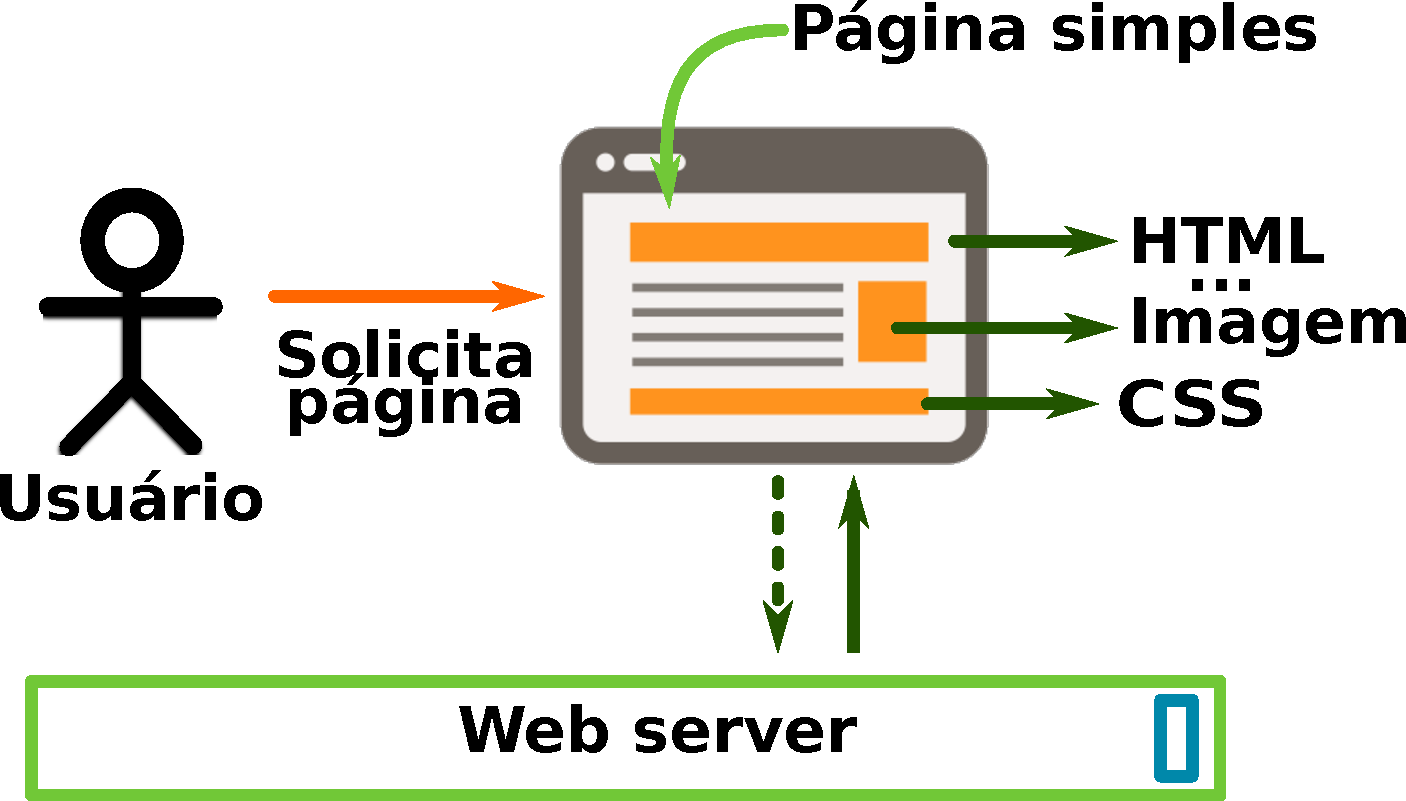
\includegraphics[width=.50\textwidth]{request_a_page}
  \caption{Do cliente para o servidor Web. Note que o navegador solicita em paralelo os damais arquivos necessários para a construção da página}
  \label{fig:client_to_web_server}
\end{figure}

A Figura \ref{fig:client_to_web_server} busca exemplificar uma situação simples
na qual o cliente solicita uma página web para um servidor. Inicialmente, o
cliente faz uma solicitação de alguma página por meio de algum software, vamos
considerar o navegador nesse exemplo. Em seguida, o navegador comunica-se com o
servidor através do protocolo HTTP; por sua vez o servidor responde devolvendo
o arquivo solicitado que contém todas as instruções básicas necessárias para
construir a página (HTML). O navegador abre o arquivo HTML retornado, converte
o conteúdo e verifica se precisa de mais informações para construir a página
solicitada; é comum que a página precise de outros arquivos como CSS, imagens,
javascript, etc. Se mais arquivos forem necessários, então o navegador solicita
os mesmos para o servidor de forma paralela ou serial. O exemplo ilustra de
forma simplificado como uma requisição acontece e como múltiplas requisições
podem ser geradas para construir uma simples tela. Um exemplo real pode ser
considerado da caracterização da carga gerada sobre o site da copa do mundo de
1998, na qual foi gerado uma média de 10796 requisições/min~\citep{worldcup}.
Um servidor web tem que responder milhares de usuários e a estrategia utilizada
para lidar com tal problema são as mais variáveis possível.

Normalmente, cada requisição feita por um cliente abre muitas conexões com o
servidor web e ao final elas são encerradas. Esse mecanismo impacta no
desempenho por duas razões: a latência aumenta e o consumo de CPU com operações
não uteis se eleva. Uma possibilidade para minimizar esses impactos é utilizar
o mecanismo de \boldAndIndex{keep-alive}, que fornece uma conexão
aberta durante as atividades dos usuários. Por exemplo, a Figura
\ref{fig:no_keep_alive} e a Figura \ref{fig:keep_alive} mostram um caso
utilizando \textit{keep-alive} e outra sem utilizar. O primeiro caso ilustra
uma situação padrão na qual uma requisição é realizada, por sua vez são abertas
e fechadas diversas conexões para obter cada um dos arquivos necessários para
construir a página. O segundo caso ilustra uma técnica chamada de
\textit{keep-alive}, cujo o objetivo é reduzir a latência e o uso de CPU no
servidor mantendo a conexão aberta por um intervalo de tempo.  Esse mecanismo
pode melhorar a experiência do usuário ao acessar o site em casos que um
servidor esteja recebendo um elevado número de requisições. Contudo, outro
aspecto do \textit{keep-alive} é que esse pode elevar o consumo de memória
gerando outro tipo de problema em um servidor sobrecarregado.

\begin{figure}[!h]
  \centering
  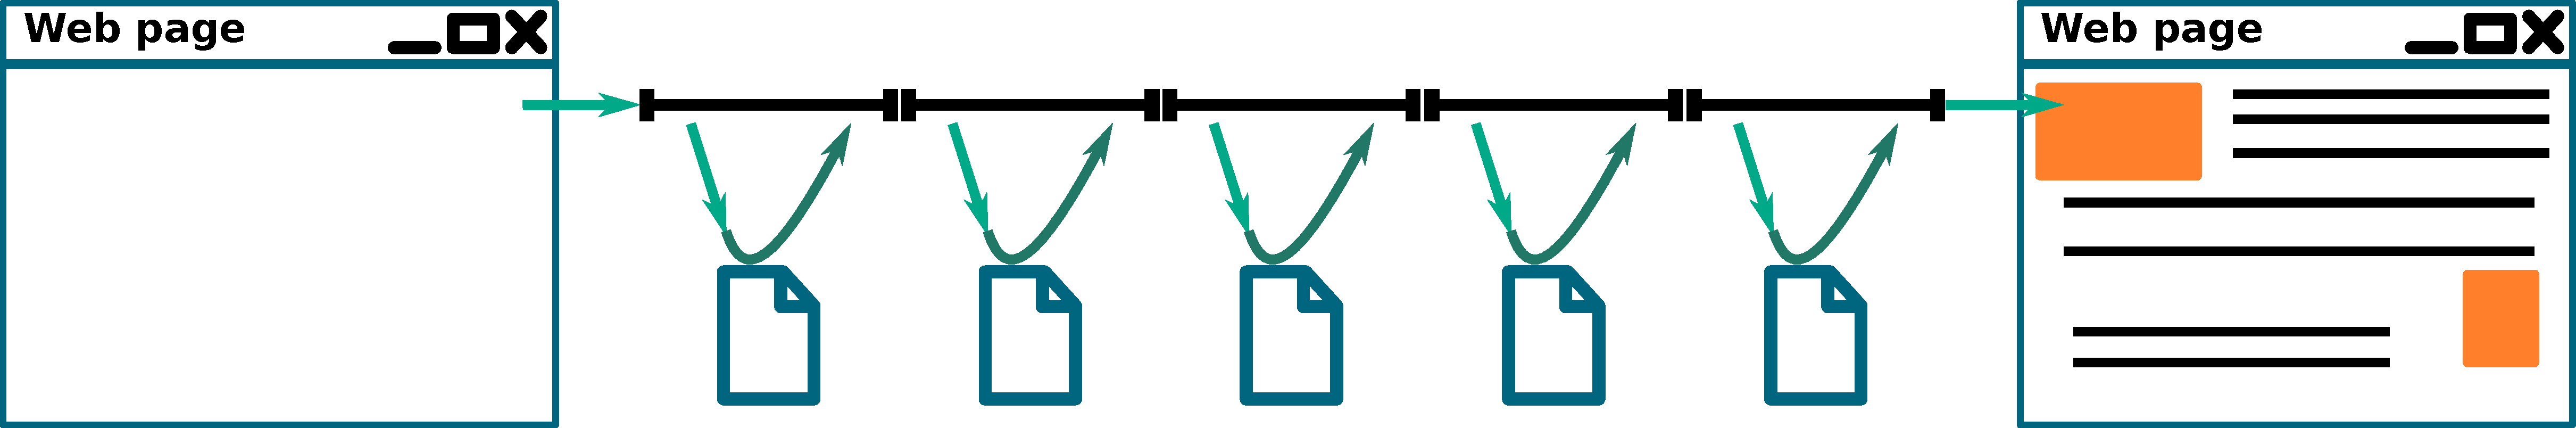
\includegraphics[width=0.8\textwidth]{no_keep_alive}
  \caption{Sem keep alive}
  \label{fig:no_keep_alive}
\end{figure}

\begin{figure}[!h]
  \includegraphics[width=0.8\textwidth]{keep_alive}
  \caption{Com keep alive}
  \label{fig:keep_alive}
\end{figure}

Existem muitos servidores web disponíveis no mercado, contudo, dois deles são
especialmente relevantes para o contexto deste trabalho:
Nginx\footnote{\url{https://www.nginx.com/}} e Apache
Httpd\footnote{\url{https://httpd.apache.org/}}.  O primeiro é conhecido pelo
seu desempenho para entregar arquivos estáticos, enquanto o segundo é conhecido
pela sua enorme estabilidade e comodidade. Ambos são extremamente
configuráveis, confiáveis e suportam grandes cargas de requisições.

\subsection{Servidor Apache HTTPD}
\label{sec:architecture}

O servidor Apache HTTPD, também conhecido como \textit{HTTP Daemon (HTTPD)} é
licenciado com a licença Apache 2.0 e mantido pela fundação Apache.  O Apache
HTTPD\footnote{Usaremos HTTPD e Apache como sinônimos nesse texto} foi
projetado para executar em vários SOs, essa restrição fez com que fosse
necessário adotar estratégias para fazer o HTTPD multiplataforma e mantendo um
bom desempenho.  Uma característica importante do HTTPD é a divisão de módulos
que manipulam processos, threads e bibliotecas portáveis utilizadas; esses
três, em conjunto, constituem a arquitetura do projeto. O Apache utiliza
a biblioteca \textit{Apache Portable Runtime (APR)} cuja a intenção é ser
utilizada como uma interface portável para as tarefas comuns de programação
(e.g.: alocação de memória, manipulação de tempo, etc). Por fim, o HTTPD
implementa um módulo especial chamado \textit{Multi-Processing Module (MPM)}
responsável por manter o processamento das requisições e a lógica de
manipulação de processos/threads. O MPM é uma boa fonte de comparação entre
diferentes modelos de processos.

\begin{figure}[!h]
  \centering
  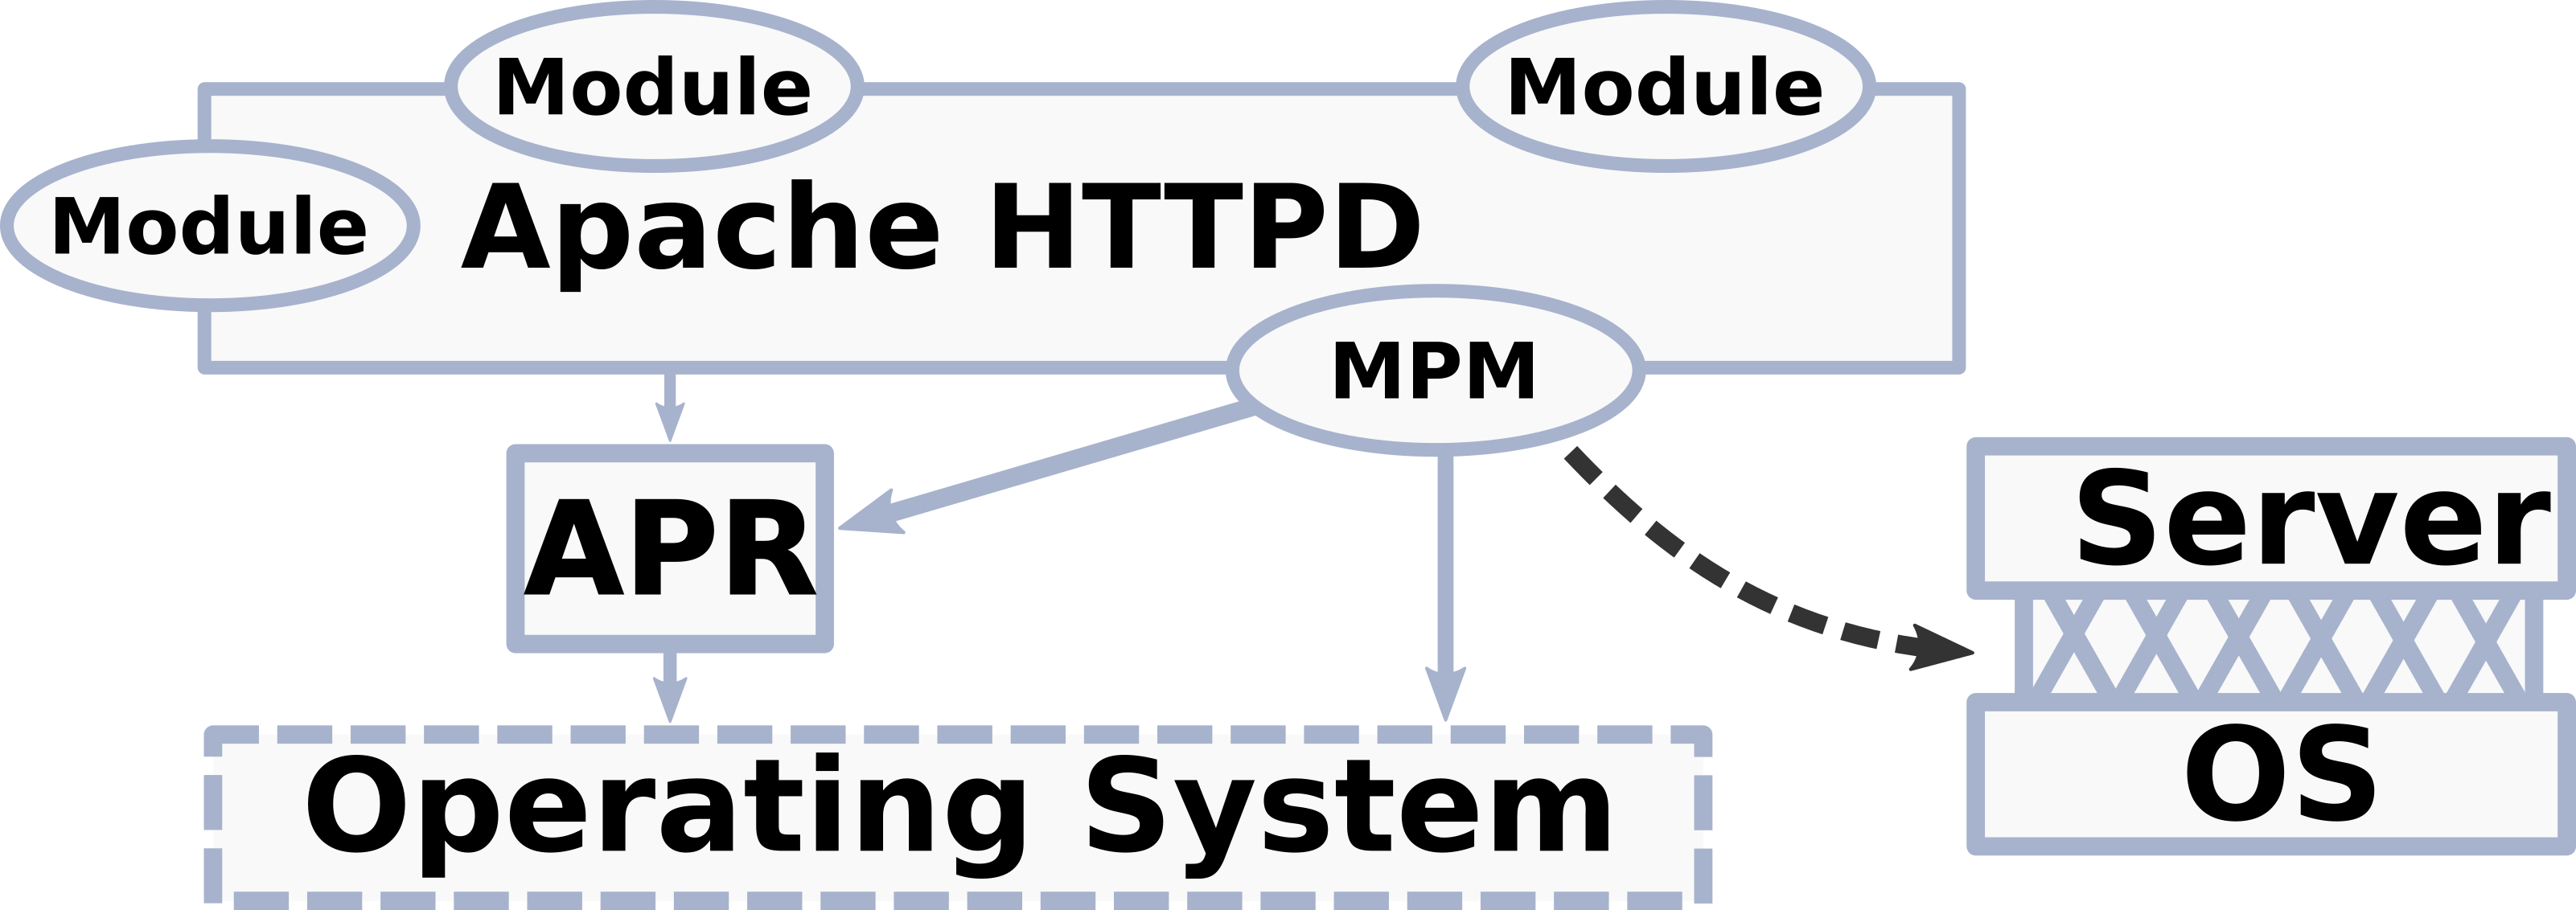
\includegraphics[width=.7\textwidth]{apache_arhitecture} 
  \caption{Arquitetura do servidor Apache HTTP \citep{apache_module_book}}
  \label{fig:apache_architecture} 
\end{figure}

A Figura \ref{fig:apache_architecture} é uma visão de alto nível da arquitetura
do Apache. O topo da imagem representa os elementos do núcleo do Apache
responsáveis por juntar os demais componentes necessários para o seu
funcionamento. Ao redor do núcleo, existe um grande número de módulos anexados
que podem ser conectados ao projeto. Esses módulos facilitam o processo de
adicionar e remover elementos do núcleo, normalmente como bibliotecas
dinâmicas. Módulos na forma de bibliotecas dinamicamente ligadas fornecem
flexibilidade, um bom desempenho e portabilidade entre diferentes SOs (e.g.; o
Window e Linux podem ter diferentes implementações para o mesmo módulo). A
Figura \ref{fig:apache_architecture} também ilustra o MPM como um componente
diretamente conectado ao SO, porque o MPM manipula os elementos de
paralelização e cada SO precisa implementar essa parte de acordo com as suas
próprias particularidades. A última parte da imagem mostra a biblioteca APR,
que se posiciona entre o núcleo do HTTPD e o SO.

\begin{figure}[!h]
  \centering
  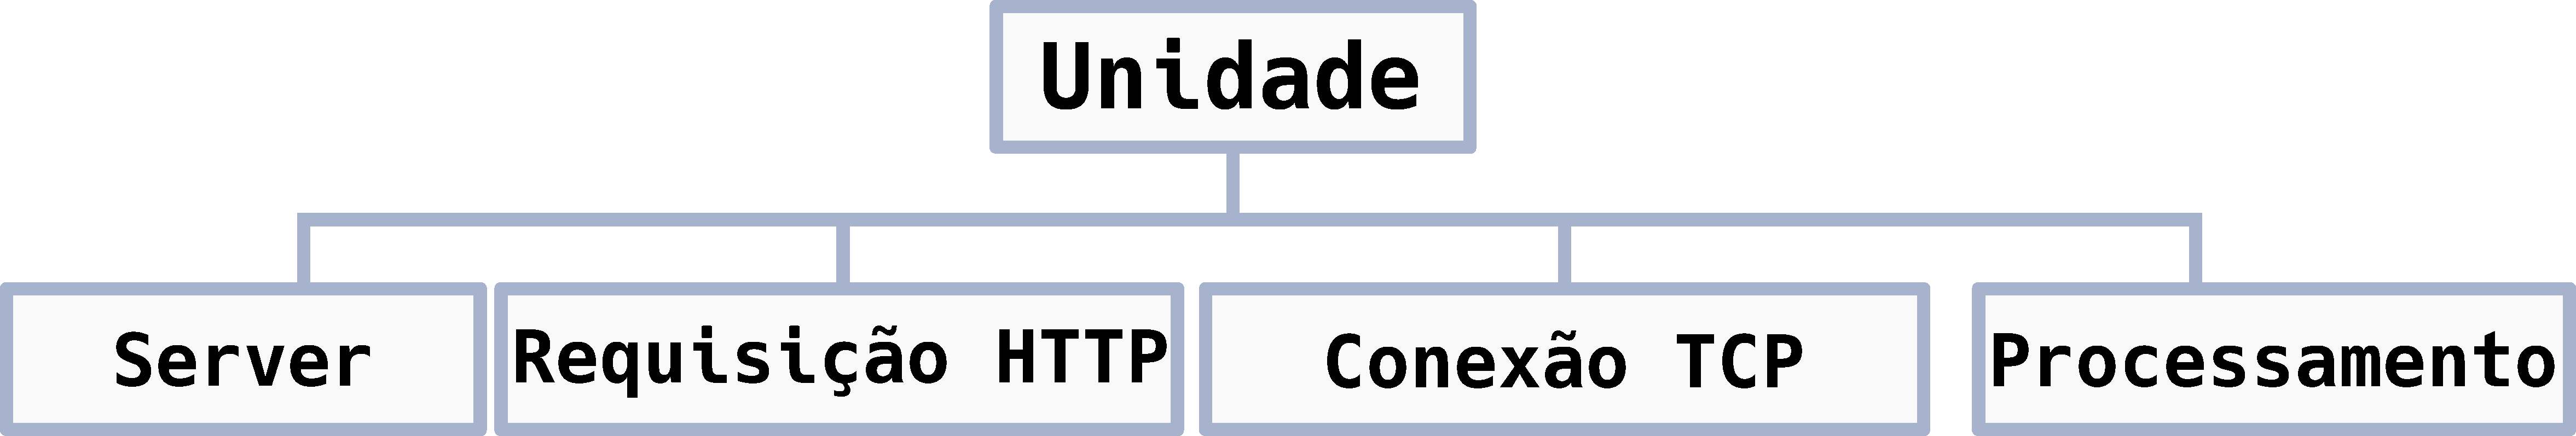
\includegraphics[width=.7\textwidth]{units} 
  \caption{Unidade do Servidor Apache HTTP}
  \label{fig:units} 
\end{figure}

Alguns módulos são essenciais para o funcionamento do HTTPD uma vez que eles
representam os elementos básicos das estruturas de dados que são usadas por
todo o código. A Figura \ref{fig:units} mostra algumas unidade fundamentais
usadas pelo HTTPD. O módulo \textit{server} é responsável por criar uma estrutura de
dados para a requisição toda vez que o HTTPD aceita uma nova conexão. O módulo
HTTP é encarregado de preencher uma estrutura de dados de requisição e o
módulo de conexão TCP constrói a estrutura de dados que mantém as informações
da conexão. Normalmente, não é preciso se preocupar com módulos relacionados
aos detalhes do HTTP, uma vez que o Apache ajusta todos os elementos necessários
e também entrega uma estrutura de dados pronta para ser utilizadas.

\begin{figure}[!h]
  \centering
  \includegraphics[width=.9\textwidth]{request_phases} 
  \caption{Gerador de Conteúdo \citep{apache_module_book}}
  \label{fig:content_generator} 
\end{figure}

Outros dois aspectos da arquitetura do Apache são o \textbf{Content Generator}
(Gerador de Conteúdo) e as fases de processamento das requisições. O
\textit{Content Generator} pode ser visto como o núcleo do Apache uma vez que
ele é responsável pelas operação de escutar por requisições e retornar
respostas; existe exatamente um gerador de conteúdo por requisição. No Apache
um módulo pode registrar um \textit{content generator} de forma simples (basta
ajustar o \texttt{httpd.conf}) e se nenhum estiver disponível o Apache utiliza
o gerador padrão que simplesmente mapeia um arquivo para uma requisição
\citep{apache_module_book}. O \textit{content generator} pode processar toda a
requisição sozinho, contudo o Apache divide a \textit{request} em várias fases
como pode ser visto na Figura \ref{fig:content_generator}. Alterações nessa
fases podem ser extremamente proveitosas para testar novas abstrações de
processos.

\subsubsection{MPM}
\label{sec:prefork}

O módulo \textit{Multi-Processing (MPM)} é um elemento especial dentro do
Apache. Como a Seção \ref{sec:architecture} introduziu, o MPM funciona como uma
interface entre o HTTPD e o SO. O MPM tem três características principais para
qualquer instância do Apache: deve ser único, é obrigatório e tem uma
implementação específica para o SO alvo. O HTTPD fornece pelo menos um módulo
MPM por SO, por exemplo, o Window utiliza \texttt{mpm\_winnt} e o Linux tem
três opções diferentes que serão tratadas em detalhes nesse trabalho. Cada uma
das três opções podem ser classificadas como baseada em processos ou em
threads, mais especificamente são elas: \textit{Prefork}, \textit{Worker} e
\textit{Event}. Esses módulos constituem bons pontos para comparar thread e
processos usando as novas abstrações, uma vez que o ambiente se conserva.

\begin{description}

	\item[Prefork:]

O \textit{Prefork} foi a primeira estratégia adotada pelo HTTPD e é totalmente
baseada em processos. A Figura \ref{fig:prefork} ilustra os três passos
realizados pelo \textit{Prefork}. O Apache inicia com um processo responsável
por gerir os filhos que serão encarregados de manipular uma requisição por vez.
Em seguida, ao receber uma requisição, o processo de controle identifica um
processo que esteja sem fazer nada e repassa a mesma para um processo filho que
se encarrega da tarefa de manipular a solicitação. Caso não exista nenhum
processo filho disponível para manipular a requisição, então o processo de
controle cria novos processos filhos. Repare que a processo de controle
comporta-se como um \textit{load balancing}.

\begin{figure}[!h]
  \centering
  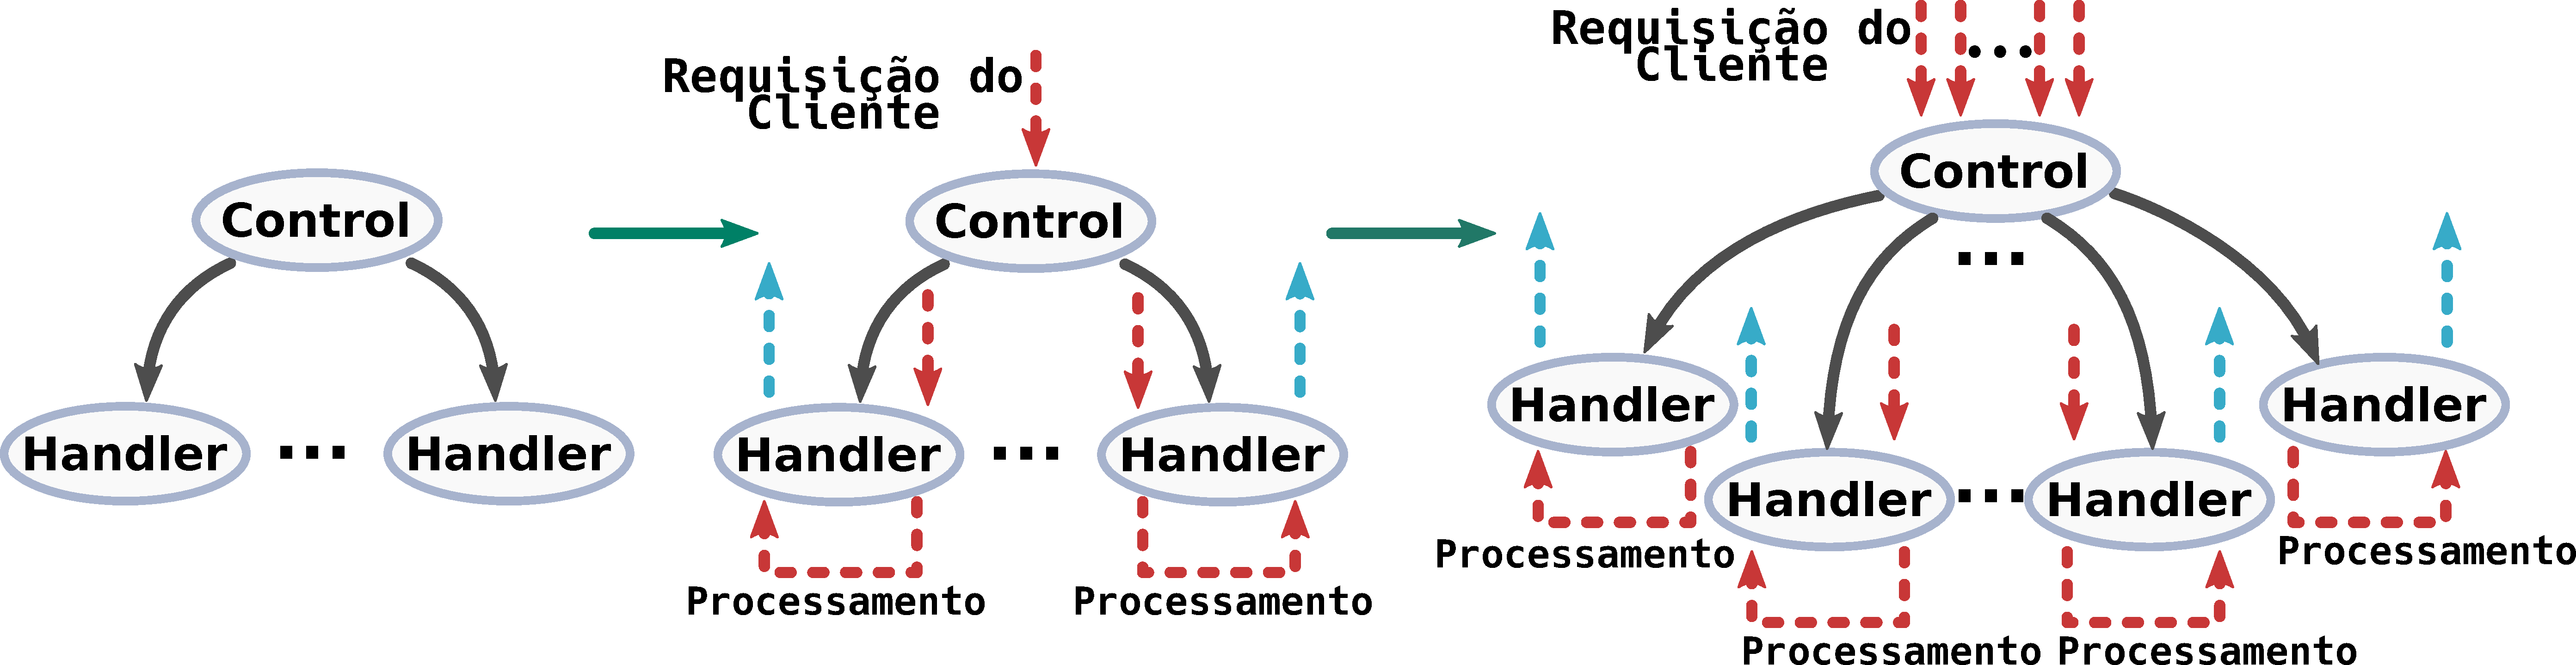
\includegraphics[width=\textwidth]{prefork} 
  \caption{Prefork}
  \label{fig:prefork} 
\end{figure}

O \textit{Prefork} é uma boa opção para servidores web que não são compatíveis
com threads (e.g., aplicações legadas escritas em PHP) e é a melhor opção de MPM
para isolar uma única requisição. Contudo, o \textit{Prefork} consome muita
memória e CPU o que não é desejável em um servidor sob forte demanda.

	\item [Worker]: O \textit{Worker} é uma solução híbrida uma vez que o seu design é baseado em
processos e threads. Esse módulo tem um processo de controle que é responsável
por criar um processos filhos e controlar o balanceamento da carga entre os
filhos. Ao contrário do \textit{Prefork}, o \textit{Worker} não cria instâncias
de processos filhos para manipular requisições feitas pelos clientes. Ele cria
diversos processos novos na qual cada um possuí várias threads para realizar a
tarefa de tratamento das requisições; comumente, o HTTPD tem que manipular uma
grande carga de requisições e nesses casos o processo de controle age criando
novos filhos (cada um com um conjunto de threads) para suportar a carga.
Repare que o \textit{Worker} utiliza threads para manipular as requisições,
isso faz com que o total de processos filhos criado seja relativamente pequeno
(comparado com o \textit{Prefork}) e consequentemente o consumo de memória
reduz. O HTTPD tem um arquivo de configuração que permite um controle fino de
todos os parâmetros relacionados ao número máximo de processos filhos, o total
de threads por filhos, o número de reposição de processos filhos e threads,
dentre outros.

\begin{figure}[!h]
  \centering
  \includegraphics[width=\textwidth]{worker} 
  \caption{Worker}
  \label{fig:worker} 
\end{figure}

A Figura \ref{fig:worker} é um exemplo de como o \textit{Worker} funciona.
Quando o Apache inicia, ele tem um processo de controle e alguns processos
filhos que mantém um grupo de threads paradas. A segunda parte da figura
representa o caso em que o HTTPD recebe um grande número de requisições e o
processo de controle cria mais filhos para suportar a carga. O \textit{Worker}
consome menos memória que o \textit{Prefork} e consequentemente ele é melhor em
casos no qual o servidor está sobrecarregado.  A mistura de processo e thread
adiciona estabilidade para todo o sistema.

	\item [Event:] O módulo \textit{Event} é baseado em threads e é o padrão na
última versão do Apache. O comportamento básico do \textit{Event} é similar ao
do \textit{Worker} com duas características a mais: \textit{keep-alive} e
separação de responsabilidade de enviar dados para o cliente. A Figura
\ref{fig:event} ilustra o comportamento básico do \textit{Event}. A forma na
qual o \textit{event} opera é similar ao \textit{worker}, com a diferença de
que ele cria um processo a mais só para manipular o envio dos dados para o
cliente.

\begin{figure}[!h]
  \centering
  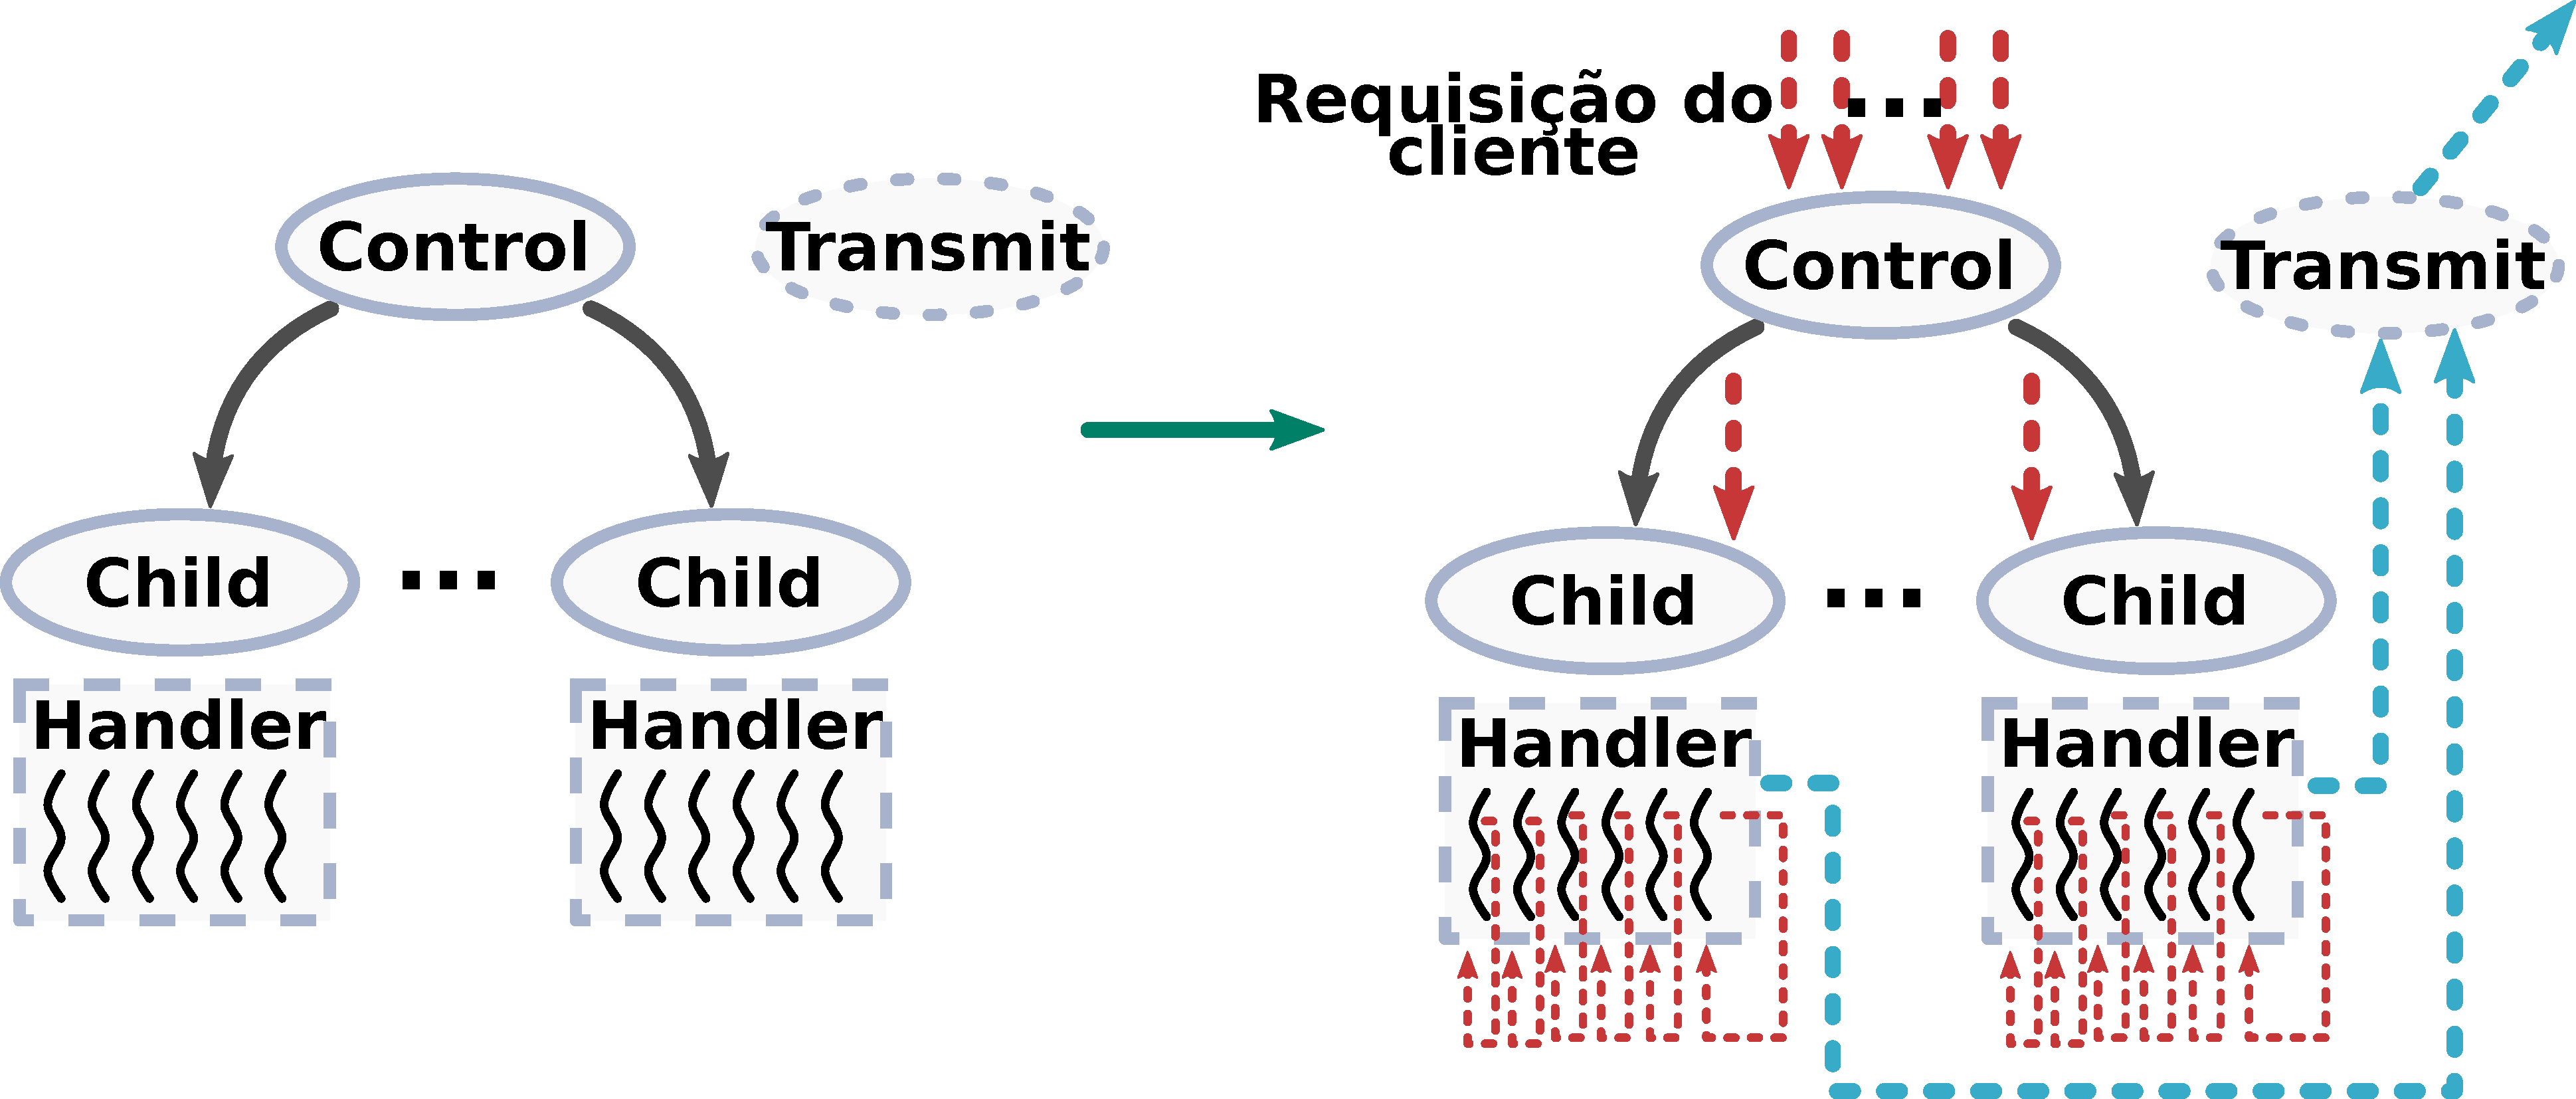
\includegraphics[width=.7\textwidth]{event} 
  \caption{Event}
  \label{fig:event} 
\end{figure}

\end{description}

\subsection{Nginx}

Assim como o Apache HTTPD o Nginx é um servidor web, contudo esse diferencia-se
de muitas formas dos servidores web tradicionais. A sua principal
característica é o seu excelente desempenho para atender requisições,
principalmente aquelas relacionadas a arquivos estáticos. Além disso o Nginx
comporta-se como um \textit{reverse-proxy}; ele recebe uma requisição do
usuário, por sua vez ele repassa a requisição para uma aplicação especifica
responsável por realizar o processamento (e.g. Puma, PHP-FPM, etc). Quando o
dado é processado pela aplicação, essa retorna o resultado para o Nginx que
repassa os dados para o usuário \citep{soni}. A Figura \ref{fig:nginx_basico}
ilustra o funcionamento geral do Nginx, note que a requisição do usuário chega
ao servidor encriptada por meio do protocolo SSL (apresentamos esse protocolo
na Seção \ref{sec:openssl}), em seguida o Nginx trata a solicitação
transformando ela em HTTP; por fim, o processo termina repassando a request
para algum serviço manipular.

\begin{figure}[!h]
  \centering
  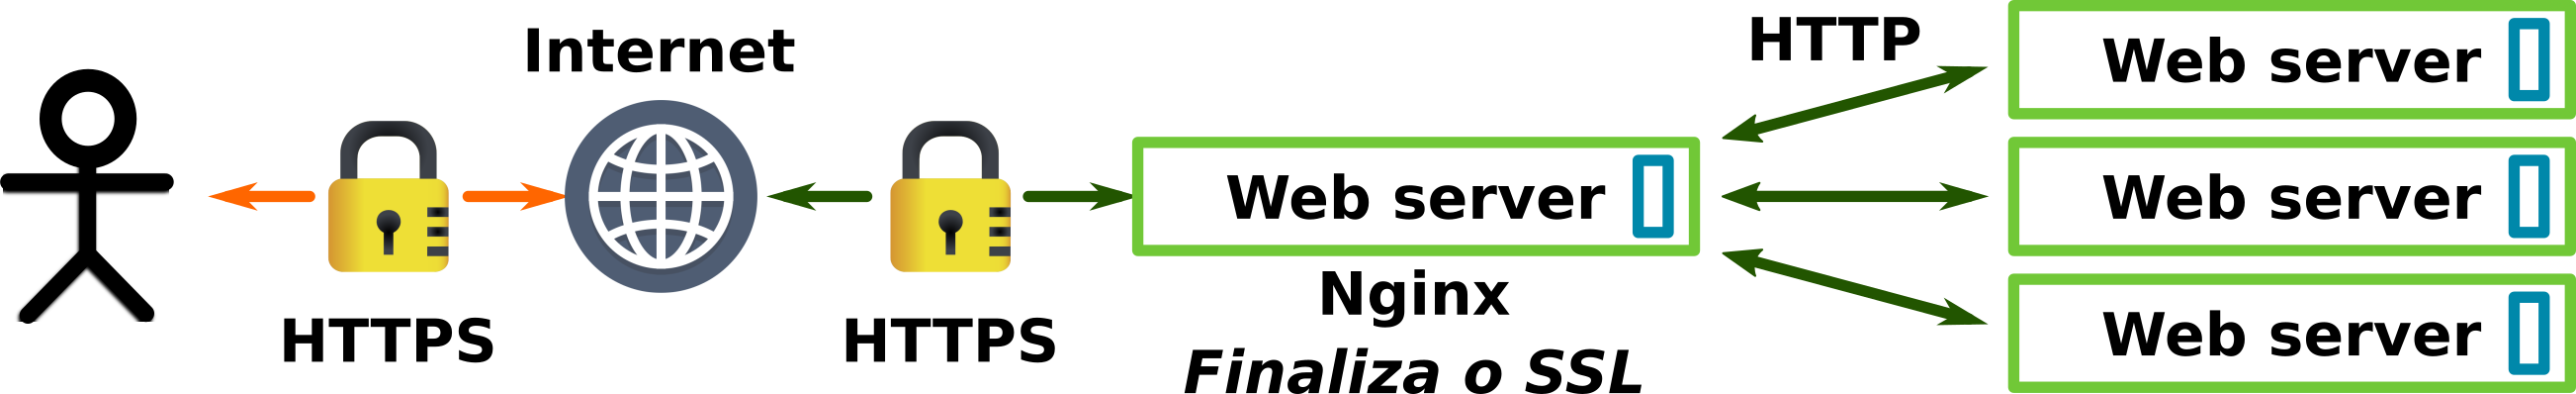
\includegraphics[width=\textwidth]{nginx_load_balancer_ex} 
  \caption{Nginx comportando-se como reverse-proxy \citep{soni}}
  \label{fig:nginx_basico} 
\end{figure}

A grande maioria dos servidores web buscam tirar o máximo de proveito dos recursos
de hardware utilizando um elevado número de threads e processos. Essa abordagem
é relativamente simples de se implementada e traz bons resultados, contudo ela
também tem alguns problemas. Dentre as desvantagens, temos que o modelo baseado
em threads/processos geram uma grande quantidade de operações que bloqueiam e
consequentemente geram trocas de contexto. Além disto, a abordagem baseada em
threads/processos consome uma elevada quantidade de recursos degradando o
desempenho da aplicação em situações de elevada demanda.

O Nginx sugere uma abordagem nova de servidor web baseada na ideia de eventos.
A estratégia de eventos parte do princípio que deve-se evitar ao máximo a troca
de contexto e assim tirar o máximo de proveito da CPU com processamento útil.
Por esse motivo o Nginx cria apenas três tipos de processos
\citep{nginx_architecture}:

\begin{itemize}
  \item Processo mestre, faz operações privilégiadas como ler arquivos de configuração e acessar portas;
  \item Processo de cache de disco, carrega dados do disco fazendo cache na memória;
  \item Processo que gerencia o cache e que realiza verificações sobre o cache periodicamente;
  \item Processos \textit{Worker} são os processos que fazem o trabalho de manipular conexões, ler e escrever em disco e comunicar-se com os servidores.
\end{itemize}

O Nginx recomenda um \textit{Worker} por núcleo da CPU, isso permite tirar
grande proveito dos eventos.

Na prática o sistema de eventos é eficiente pois gera poucos bloqueios
(comparado com o modelo que utiliza threads/processos) uma vez que esse não
espera a aplicação terminar o que está fazendo. Por exemplo, se o
\textit{worker} estiver atendendo uma requisição e em um determinado momento
precisar recuperar uma informação do disco, o \textit{worker} não bloqueia, ele
simplesmente vai fazer outra tarefa e salva o evento referente a busca no disco
para retornar nele depois (mais precisamente, quando surgir um evento). O
sistema de eventos faz com que um único \textit{worker} execute múltiplas
tarefas de forma sequencial sem bloqueio e consequentemente com poucas trocas
de contexto.

\section{Ferramentas de Comunicação Encriptada}
\label{sec:com_enc}

Como mostrado no Capítulo \ref{cap:trabalhos-analisados}, algumas das novas
propostas de abstrações de processos levam melhorias de segurança para o espaço
de usuário. Nesse sentido aplicações que envolvem mecanismos de encriptação ou
que buscam levar algum nível de segurança, representam bons casos de uso para
validar novas abstrações. Esse tipo de software costuma ser desenvolvido por
uma comunidade de especialistas na área de segurança, o que significa que levar
melhorias nesse tipo de ferramenta não é uma tarefa trivial. Essas
características fazem com que esse tipo de aplicação representem bons caso de
validação para novas abstrações de processos. Por uma questão de simplicidade e
abrangência escolhemos duas ferramentas amplamente utilidades: OpenSSH e
OpenSSL.

\subsection{OpenSSL}
\label{sec:openssl}

Antes de discutir sobre o OpenSSL é importante apresentar de forma geral o
protocolo \boldAndIndex{Secure Sockets Layers (SSL)}. O principal objetivo do
SSL é fornecer um conjunto de protocolos criptográficos que permita a
comunicação segura na rede. Basicamente, esse constituí uma ferramenta de uso
cotidiano, tendo diversas aplicações de missão crítica dependendo de tal
protocolo o que faz dele um constante alvo de ataques.

O SSL utiliza um mecanismo chamado de \boldAndIndex{handshake} que
nada mais é do que um processo de negociação entre o cliente e o servidor de
forma a criar uma conexão segura entre ambos, a Figura
\ref{fig:openssl_handshake} descrever de forma geral os passos da negociação. O
processo de \textit{handshake} começa com o cliente mandando uma mensagem do
tipo "Oi, sou o cliente" para o servidor; nessa mensagem o cliente informa a
versão do SSL que está usando, os algoritmos de criptografia e os métodos de
compressão que ele sabe manipular. O servidor por sua vez manda um "Oi, sou o
servidor" dizendo qual algoritmo usar (selecionado da lista que o cliente
mandou), um ID da seção, um certificado digital e a sua chave pública. Com o
certificado, o cliente consulta uma \textit{Certificate Authority (CA)}
(Autoridade Certificadora) que valida se o servidor é valido ou não, isso serve
para estabelecer a confiança sobre o servidor. Depois que o cliente recebe a
validação da CA, ele começa a etapa de troca de chaves na qual o cliente envia
a chave secreta compartilhável. O cliente criptografa tal chave com a chave
pública fornecida pelo servidor e o cliente termina enviando uma mensagem de
fim. O servidor desencripta a mensagem do cliente e utiliza a chave enviada
para criptografar uma mensagem de fim para ser enviada para o o cliente. Quando
o \textit{handshake} termina, o servidor e o cliente podem enviar mensagens que
são simetricamente encriptadas \citep{openssl}.

\begin{figure}[!h]
  \centering
  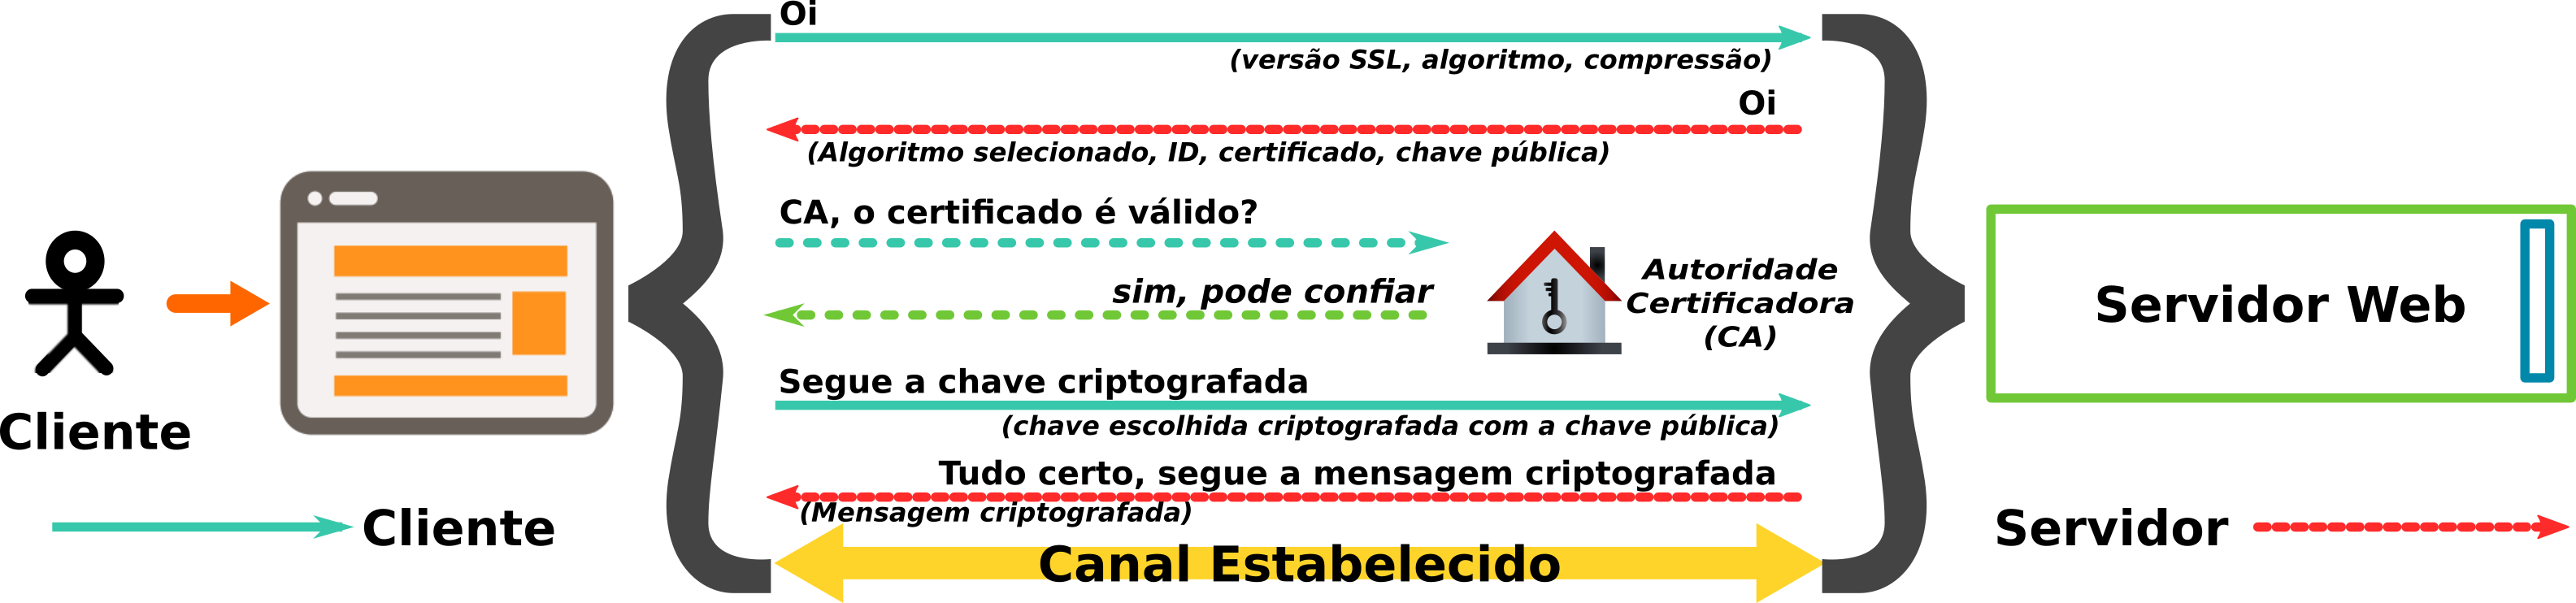
\includegraphics[width=\textwidth]{ssl_handshake}
  \caption{Do cliente para o servidor Web}
  \label{fig:openssl_handshake}
\end{figure}

O OpenSSL é uma implementação livre do protocolo SSL, ele contém a
implementação de várias funções criptográficas e utilitárias. A Figura
\ref{fig:openssl_arch} mostra uma visão geral da arquitetura do OpenSSL. O
\textit{EVP crypto API} são funções de alto nível que fornecem recursos para
derivação de chaves, hash seguro, código de autenticação de mensagens,
encriptação/decriptação de algoritmos simétricos/assimétricos, dentre outros. A
arquitetura também fornece uma pilha de manipulação de erros e uma interface
abstrata para lidar com I/O.

\begin{figure}[!h]
  \centering
  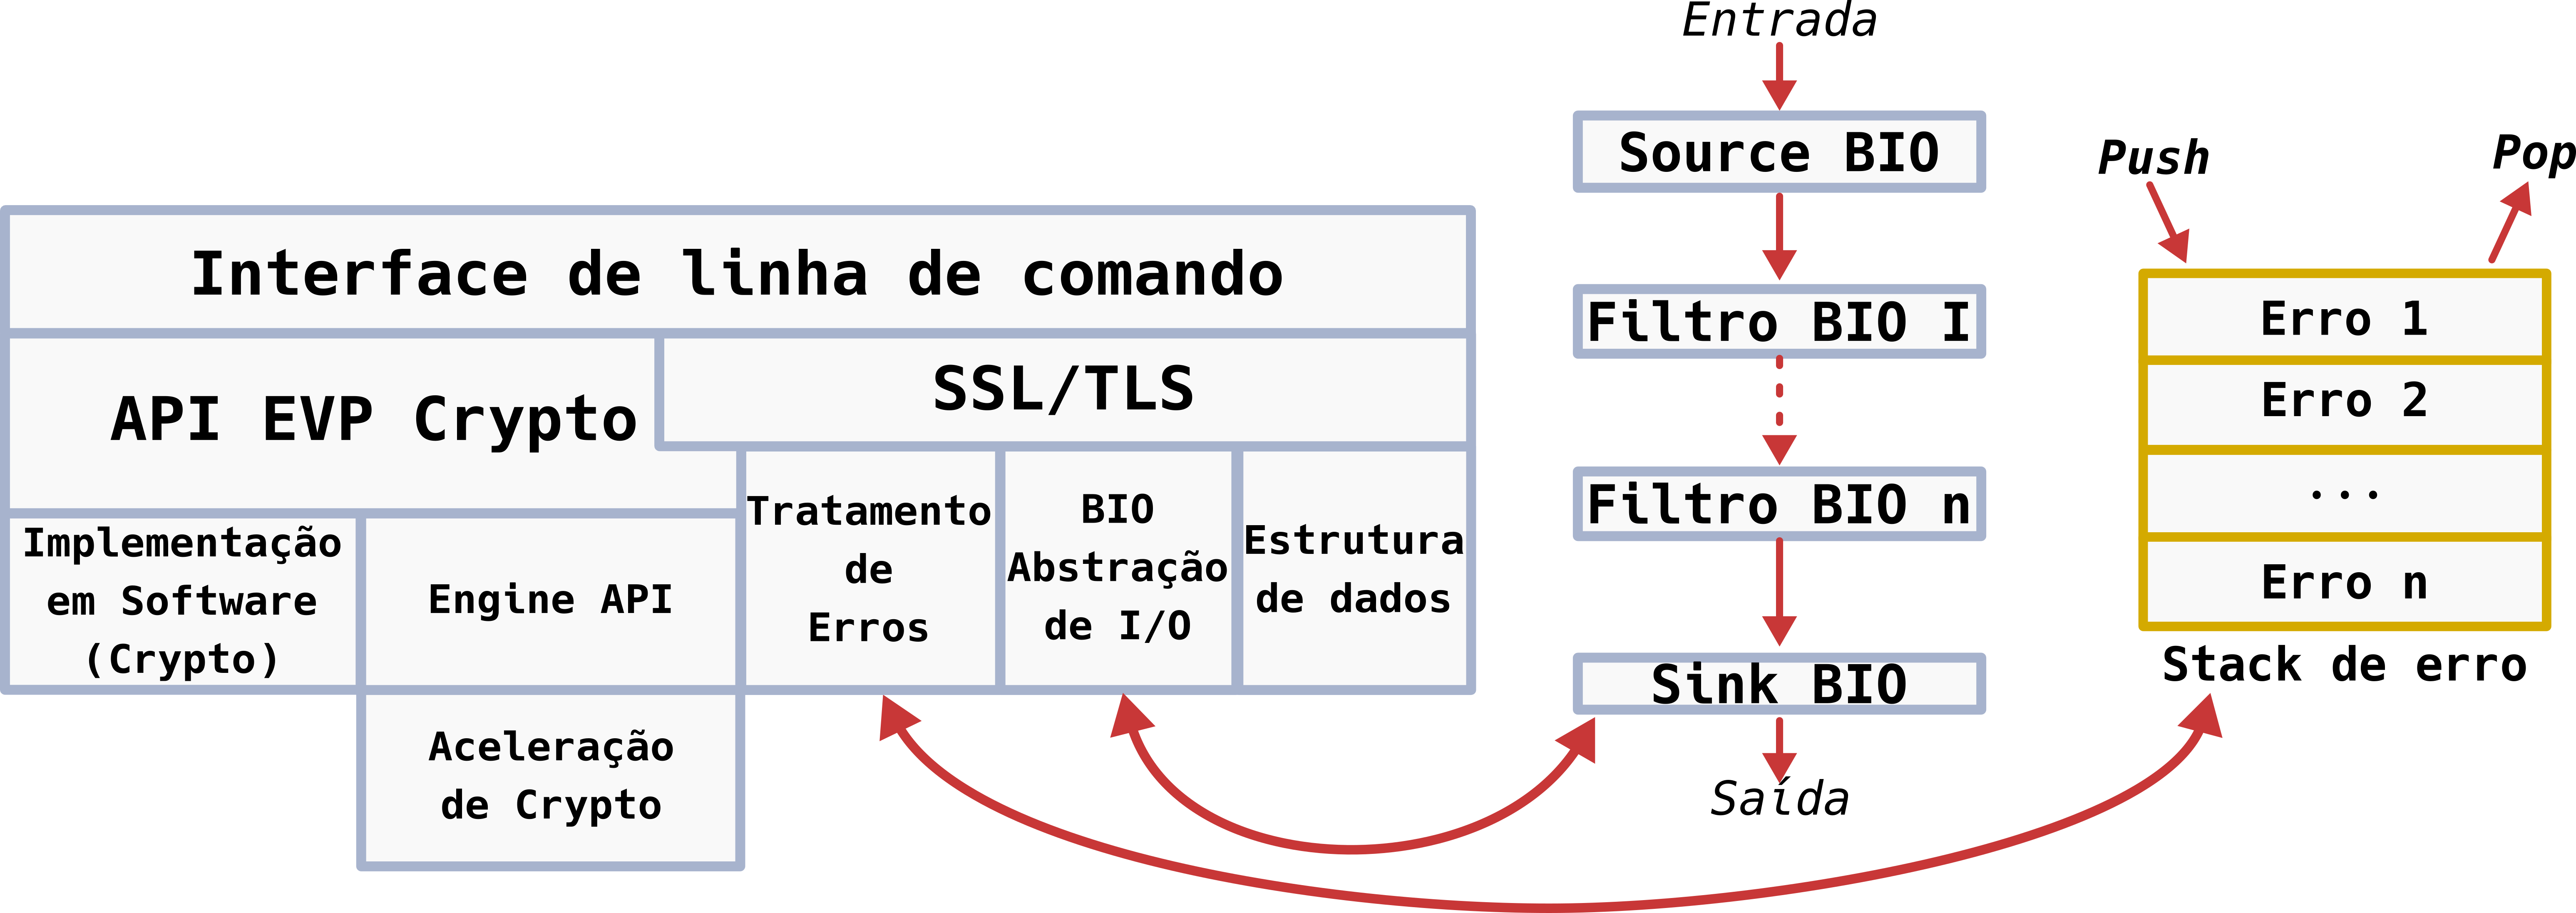
\includegraphics[width=\textwidth]{openssl_arch}
  \caption{Arquitetura do OpenSSL \citep{crypto_openssl}}
  \label{fig:openssl_arch}
\end{figure}

\subsection{OpenSSH}

Uma das tarefas mais comuns do dia-a-dia de muitos desenvolvedores consiste em
acessar servidores em diversos locais do mundo e configurar uma determinada
aplicação. Na prática, boa parte dos profissionais de TI faz uso de conexões
seguras na Internet por meio do protocolo \textit{Secure Shell (SSH)}. Existem
diversas implementações desse protocolo, mas para este trabalho discutiremos o
OpenSSH.

A Figura \ref{fig:openssh_layer} apresenta uma visão geral da arquitetura do
OpenSSH. Primeiramente repare que as três camadas correspondentes as camadas
SSH encontram-se sobre a camada TCP/IP que consistem em uma conexão não segura.
A primeira camada se chama \textit{ssh-transport} e ela é responsável por
realizar operações criptográficas, proteção contra ataques e reverificar chaves
de tempos em tempos. Logo após a primeira camada temos o \textit{ssh-userauth}
que é responsável pela autenticação, se tudo der certo durante a autenticação,
então a troca de chaves acontece e a conexão segura é estabelecida. Por fim a
camada \textit{ssh-connection} estabelece um canal seguro e fica responsável
por gerir a multiplexação de múltiplas conexões e redirecionamentos
\citep{proopenssh, opensshhood}.

%TODO: CVE
\begin{figure}[!h]
  \centering
  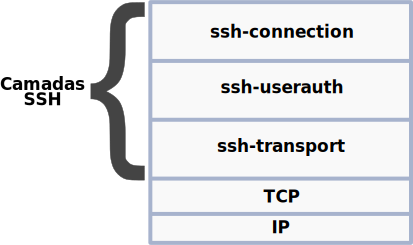
\includegraphics[width=0.3\textwidth]{ssh_layers}
  \caption{Camadas SSH \citep{opensshhood}}
  \label{fig:openssh_layer}
\end{figure}

Dado a enorme importância do OpenSSH, esse é alvo de constantes ataques e
consequentemente recebe diversos aprimoramentos. Como resultado, algumas CVEs
foram criadas e resolvidas no OpenSSH. Dentre as CVEs destacamos: TODO :(

% TODO: Destacar

Do ponto de vista do uso de tal aplicação para validar propostas de abstrações
de processos, destacamos que essa pode ser usada para demonstrar ganhos de
segurança e controle de acesso a memória. Uma abordagem é partir de uma versão
antiga do OpenSSH que não tem a correção para alguma vulnerabilidade e
demonstrar que a nova abstração sugerida consegue resolver o problema. Note que
os pontos mais fracos do OpenSSH podem ser destacados:

\begin{itemize}
  \item Acesso a chave é uma região crítica e deve ter o seu acesso restrito;
  \item Potencial vazamento de dados;
  \item Escalada de privilégios.
\end{itemize}

\section{Outras Aplicações para Avaliar Diferentes Aspectos}

As propostas de novas abstrações de processos podem levar benefícios para
outras áreas além das mostradas nas Seções \ref{sec:web_server} e
\ref{sec:com_enc}. Por esse motivo, apresentamos algumas ferramentas que são de
ampla utilização no mercado e que podem ser utilizadas na validação da
utilidades de algumas das novas abstrações sugeridas.

\subsection{Redis}

Escalar alguns sistemas não é uma tarefa trivial e exige constantes
customizações. Como resultado dessa necessidade, surgiu o sistema Redis que
consiste da ideia de utilizar um sistema que pode ser um cache e ao mesmo tempo
um sistema de armazenamento utilizando a memória principal (RAM) com o objetivo
de levar ganhos de desempenho para a aplicação. O Redis também salva os dados
da memória para o disco, isso permite que posteriormente ele consiga
reconstruir o sistema na memória.

O Redis é famoso por utilizar como forma de armazenamento o esquema de
chave-valor (\textit{key-value}). Essa técnica permite o armazenamento dos dados na
forma de um par que consiste de uma chave identificadora e um valor associado a
chave. Quando um valor-chave é salvo, isso significa que o par está presente na
RAM, no Redis, uma chave tem que ser uma string mas seus valores podem ser de
vários tipos diferentes, dentre as abstrações de dados suportadas destacam-se:

\begin{itemize}
  \item Lista de strings
  \item Conjunto de strings
  \item Conjunto de strings ordenadas
  \item Tabelas de hash na qual a chave e valor são strings
  \item HyperLogLogs
  \item Stream de entradas com grupos de consumidores
  \item Dados Geoespaciais
\end{itemize}

O tipo utilizado no valor determina qual operação é possível de ser aplicada.
De forma geral o Redis permite realizar operações de alto nível (e.g.,
operações do lado do servidor, uniões e diferenças).

A Figura \ref{fig:redis} apresenta uma visão de geral da organização do Redis.
Repare que o Redis fornece uma interface de interação do lado do cliente (via
linha de comando ou API) e possui um servidor que é responsável por lidar com
os dados.  O servidor é responsável por gerir os dados na memória e em disco,
por isso a sua implementação faz constante uso da criação de processos (via
chamada de sistema \texttt{fork()}). Basicamente, toda vez que um armazenamento
é necessário, o Redis faz um \texttt{fork()} do processo pai, em seguida o
processo filho da início ao processo de escrita em disco enquanto o processo
pai continua realizando as suas tarefas. 

\begin{figure}[!h]
  \centering
  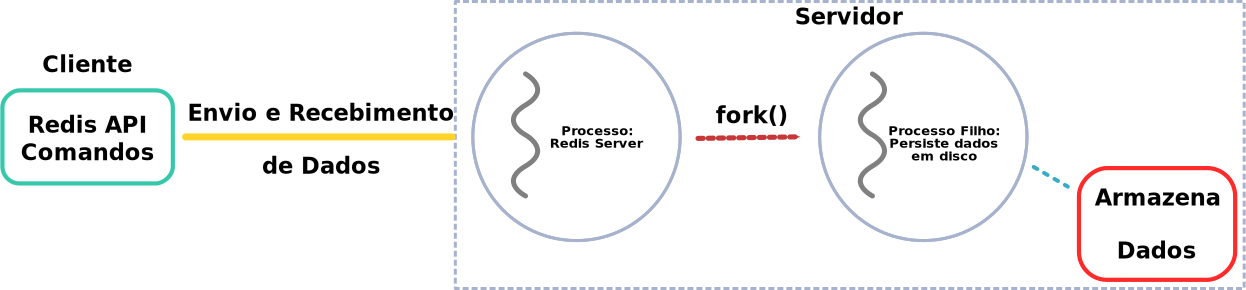
\includegraphics[width=\textwidth]{redis_overview}
  \caption{Visão geral do funcionalmento do Redis}
  \label{fig:redis}
\end{figure}

Um dos aspectos mais interessante do Redis, da perspectiva das novas abstrações
de processo, é a persistência dos dados. O Redis fornece três formas
\citep{redisio}: \textit{Relational Database (RDB)}, \textit{Append-Only-File
(AOF)} e comando SAVE. O RDB faz uma cópia de todos os dados presentes na
memória para o disco, por padrão, o Redis escreve os dados a cada dois
segundos. Repare que o RDB pode causar perda de dados em caso de mal funcionar,
uma alternativa seria configurar o Redis para fazer mais escritas, contudo isso
eleva consideravelmente o consumo de memória pela natureza do uso de
\texttt{fork()}. O AOF registra todas as operações de escritas feitas pelo
servidor, logo tudo é persistido. O AOF tem o problema de que pode ser mais
lento do que o RDB a depender da política de sincronização adotada e também
consumir mais memória.  Por fim o comando SAVE força o servidor a criar um
\textit{dump} dos dados no momento em que foi solicitado.

% TODO: Vale a pena dar um certo nível de detalhes do código? Não é tão complicado fazer isso, mas preciso ter certeza antes se vale a pena
% Além da referencia do "Redis: under the hood" tem esse artigo aqui: http://robertlehmann.de/img/redis.pdf

\subsection{Garbage Collection (GC)}

Várias linguagens de alto nível possuem mecanismos de gerenciamento recursos
(e.g., memória, processamento paralelo, datas, etc) que garantem a portabilidade
da aplicação e removem a complexidade de ter que gerenciar recursos de baixo
nível. Dentre as vantagens de tais tecnologias, destacam-se o fato de que o
programador pode manter o foco nas características da aplicação e também reduz
a chances de erros graves. O Java é o principal representante desse tipo
linguagem, fornecendo mecanismos de gerenciamento automático da memória e sendo
portável para múltiplas plataformas. Por uma questão de simplicidade, iremos
adotar o Java para as discussões desta seção. Todas as flexibilidades
oferecidas pelo Java deve-se ao uso da \textit{Java Virtual Machine} (JVM) que
fornece elementos para a manipulação dos recursos do SO. Um dos principais
elementos da JVM é o \textit{Garbage Collection} (GC), cujo a principal tarefa
consiste em abstrair o gerenciamento de memória da aplicação de forma que ela
não tenha que lidar com tal aspecto (alocar e desalocar). Dado o seu impacto, o
GC tem sido alvo de constantes otimizações ao longo dos anos e esse é um
elemento que pode se beneficiar de novos recursos oferecidos por extensões
abstrações de processos.

O GC é uma aplicação que é parte da JVM executando junto com a aplicação.
Independentemente do algoritmo de gerenciamento de memória implementado pelo
GC, todos eles definem o termo \boldAndIndex{Stop the World (STW)} ou
\textit{Parar tudo} \citep{gc_pauseless}. O STW é uma operação realizada pela
JVM  na qual todas as threads da aplicação são suspensas para que o GC execute,
em outras palavras, a única thread executando será a do coletor. Note que o GC
requer pausa para funcionar, isso é preciso pois seus algoritmos precisam que
aplicação não faça nenhuma atualização da memória durante uma das fases do
processo de limpeza da memória.

Existem diversos algoritmos que podem ser adotados pelo GC, contudo podemos
generalizar três etapas gerais: \textit{Marking}, \textit{Sweep} e
\textit{Compact}. A etapa de \textit{Marking}, também conhecida por pintura,
consiste em inspecionar os objetivos na memória para verificar quais ainda são
considerados vivos. Para determinar se um objeto está vivo o GC começa por
lementos conhecidos como objetos raiz ou \textit{Garbage Collection Roots}, os
seguintes componentes são considerados como um GC root: variáveis locais,
entrada de parâmetros, threads ativas, campos estáticos e referências JNI
\citep{gc_basics}. Partindo de um GC root, o GC atravessa o grafo dos objetos
alcançáveis e para cada elemento que consegue acessar ele “pinta” a referência
como viva. A Figura \ref{fig:gc_alg} ilustra o algoritmo descrito. No contexto
do GC, o processo de parar as threads para que a JVM possa executar a etapa de
\textit{Marking} recebe o nome de \textit{safe point} (ponto seguro) e essa
gera um STW. O tamanho da pausa é definido pela quantidade de objetos
alcançável e o seu tamanho no \textit{heap}.

\begin{figure}[!h]
  \centering
  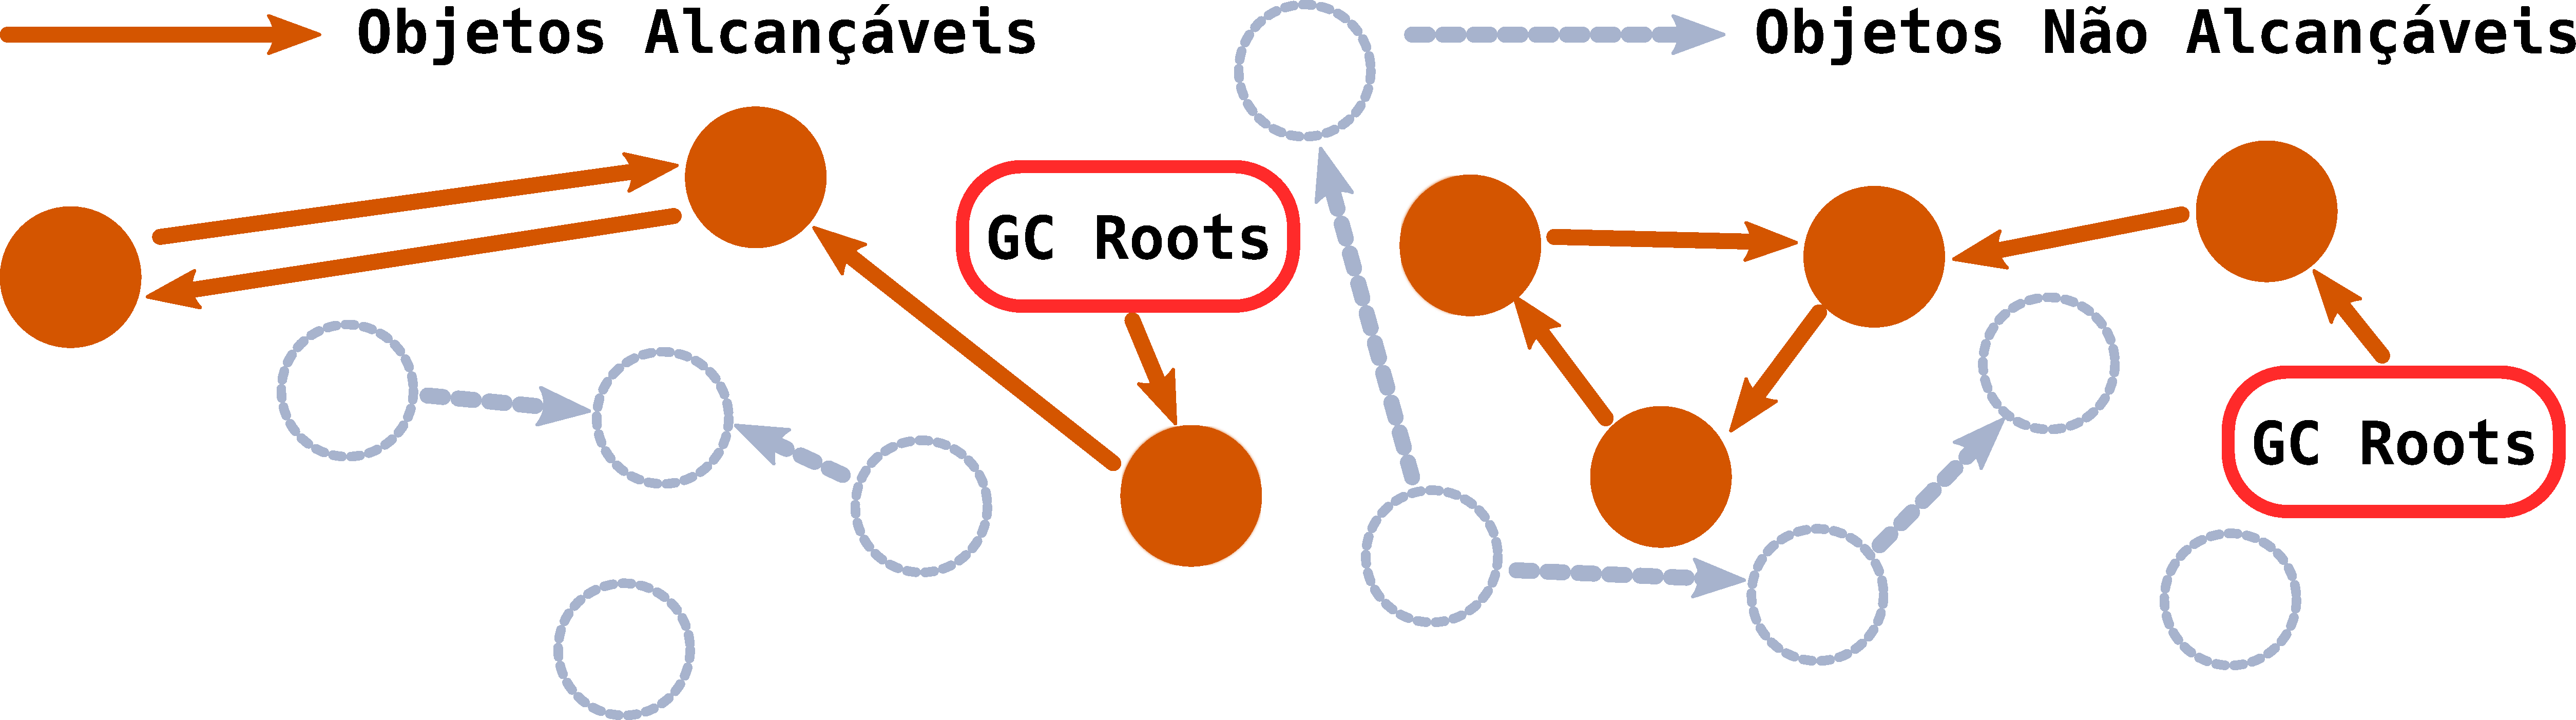
\includegraphics[width=\textwidth]{gc_algoritmo}
  \caption{Algoritmo de pintura da memória\citep{gc_basics}}
  \label{fig:gc_alg}
\end{figure}

Depois da etapa de pintar os objetos na memória, entra em ação a etapa de
remover os objetos que não foram pintados; note que essa etapa pode acontecer
em paralelo ou não, depende do algoritmo adotado. O processo de remoção pode
gerar fragmentação na memória, o que pode representar um problema uma vez que o
GC pode não encontrar espaços de memória grande o suficiente para outros
objetos. Por isso também existe uma fase de compactação na qual o GC realoca os
objetos pintados para liberar espaço contíguo. Contudo, para que a compactação
aconteça corretamente as referências dos objetos tem que ser atualizadas uma
vez que a posição física dos objetos mudou. O processo de atualizar as
referência chama-se remapeamento e ele precisa examinar toda a memória para
realizar os ajustes, note que a etapa de compactação eleva o tempo de STW. A
Figura \ref{fig:gc_mem} apresenta uma visão da memória durante as três etapas
descritas.

\begin{figure}[!h]
  \centering
  \includegraphics[width=0.8\textwidth]{gc_memory}
  \caption{Visão da memória durante a aplicação do algoritmo de GC\citep{gc_basics}}
  \label{fig:gc_mem}
\end{figure}

Vale salientar que existem diversos algoritmos de GC, cada um com suas
vantagens e desvantagens; nosso objetivo nessa seção é apenas ilustrar o
potencial de uso de tal aplicação para validar novas abstrações de processos.

\section{Discussão Sobre as Aplicações}
\label{sec:disc_app}

Desde o começo deste capítulo até está seção apresentamos algumas aplicações
destacando o seu funcionamento, estruturas básicas e os recursos exigidos por
elas. Contudo, o nosso principal objetivo é verificar quais tipos de benefícios
e validações que tais aplicações podem fornecer para o avanço das pesquisas em
novas abstrações de processos. Cada tipo de aplicação pode ser útil para
demonstrar algum aspecto da nova abstração, mas idealmente é interessante
evidenciar que as demais aplicações apresentadas também não sofrem com a nova
abstração.

O Apache e o Nginx são aplicações cujo o objetivo é servir requisições feitas
pelos usuários, ou seja, são servidores web. Esse tipo de aplicação normalmente
oferece opções para que sejam amplamente configuradas de forma a atender os
requisitos do usuário da melhor maneira possível. Tais aplicações são
especializadas para tirar o máximo de proveito possível dos recursos de hardware,
uma vez que servidores web podem lidar com enormes cargas de requisições
levando a um ostensivo uso do hardware. Nesse tipo de aplicação é comum que
ocorra um amplo consumo da memória e que a CPU esteja próxima do 100\% de
utilização em situações estresse (muitos usuários acessando).  Note que quanto
mais tempo uma requisição vive, mais memória é consumida, por isso é desejável
que as requisições sejam atendidas o mais rapidamente possível. Por sua vez o
SO tem que manipular diversos aspectos relacionados a memória, processos e
arquivos. Por esse motivo, utilizar esse tipo de software como prova de
conceito para demonstrar a eficácia de uma nova abstração de processos é algo
extremamente desejável. Essas aplicações podem ser utilizadas para mostrar que
o comportamento da alteração na abstração de processos em uma situação de alta
demanda. Contudo é importante ressaltar que os testes realizados em tais
ferramentas devem gerar uma carga substancial para que a configuração padrão
tenha que ser alterada. Esse aspecto é fundamental uma vez que não existe
grande valor em demonstrar algo usando tais ferramentas com uma carga pequena,
pois isso pouca ajuda na verificação dos reais impactos gerados pela nova
extensão do processo.

O Apache também possuí um ambiente que permite testar processos e threads de
forma equivalente. Tal característica é interessante para comparar novas
abstrações diante de dois modos de execução amplamente utilizados. De forma
similar o Nginx usa outro modelo chamado de \textit{event} que também
representa outra contexto para validação. Da forma como o Apache e o Nginx
manipulam requisições, podemos dizer que o primeiro fornece um isolamento
horizontal enquanto o segundo proporciona isolamento vertical. O isolamento
horizontal vem do fato de que um processo cria vários outros e o vertical vem
da criação de um único processo por núcleo do processador durante a
inicialização. Esses dois níveis de isolamento podem ser úteis para demonstrar
que uma nova abstração pode melhorar o isolamento sem degradar o desempenho.

O Apache trabalha com diversos \textit{plugins} que são acoplados ao código
principal dinamicamente. Essa junção tem uma boa relação desempenho e
flexibilidade, mas também elevam as chances de quebrar o Apache.  Portanto o
sistema de \textit{plugins} do Apache fornece um bom elemento de validação para
aquelas abstrações que visam trazer isolamento e recuperação.

Várias propostas de extensão da abstração de processos sugerem algum ganho de
segurança por meio do controle fino ou isolamento de pedaços da memória. Nesse
sentido o OpenSSH e OpenSSL são ferramentas interessantes, já que possuí os
requisitos de segurança adequado para a validação das novas abstrações. Em
especial, ambas as aplicações tem diversas CVEs associadas a si com correções
disponíveis a partir de uma versão especifica. Portanto uma proposta de
melhoria na abração de processo que eleva a segurança pode demonstrar o seu
real valor em uma dessas aplicações.

O Redis por sua vez é uma aplicação que trabalha com grandes quantidade de
dados na memória e que tem um excelente desempenho em situações de forte
demanda. Essas características fazem do Redis uma excelente ferramenta para
demonstrar novas técnicas de compartilhamento da memória. Além disso, um dos
objetivos do Redis é auxiliar na escalabilidade das aplicações por isso é
desejável que o mesmo reaja rapidamente a qualquer problema. Nesse contexto,
abstrações de processos novas que tragam melhorias no tempo recuperação de uma
aplicação em caso de falha podem usar o Redis com instrumento de validações.

Novas abstrações de processos podem entregar ganhos de desempenho para as
aplicações por utilizar algum recurso de hardware ou mesmo fornecer uma nova
estrutura de dados para a aplicação. Tal otimização pode ser demonstrada em um
GC uma vez que esse tipo de aplicação faz uso de vários algoritmos que dependem
de certos dados fornecidos pelo SO. Como exemplo disto, a fase de compactação
pode ser otimizada se o endereço virtual for mantido e apenas o endereço físico
alterado \citep{pauseless}.

A Tabela \ref{tab:app_alvos} busca resumir quais aplicações podem ser usadas
para demonstrar algum aspecto da nova abstração de processos. Além disso essa
seção inteira responde a pergunta RQ3 uma vez que apresenta e discute diversas
aplicações. Por fim repare da Tabela \ref{tab:app_alvos} que o Apache é uma das
ferramentas que melhor pode ser usada para demonstrar os aspectos de uma nova
abstração de processos. No Capítulo \ref{cap:estudo-de-caso} aprofundamos a
validação utilizando o Apache para testar o MVAS. 

\begin{table}[]
\small
\centering
  \begin{tabular}{|@{}c@{}|@{}c@{}|@{}c@{}|@{}c@{}|@{}c@{}|@{}c@{}|@{}c@{}|}
  % TOPO DA TABELA
  % |M{2.5cm}|M{2.5cm}|M{2.5cm}|
  \hline
  \multicolumn{1}{|l|}{\diagbox[width=2.5cm, height=2cm]{App}{Alvo}} &
    % Troca de contexto
    \multicolumn{1}{@{}c@{}|}{\begin{tabular}[c]{@{}c@{}}Controle\\fino da\\Memória\end{tabular}} &
    % Persistência de processos
    \multicolumn{1}{@{}c@{}|}{\begin{tabular}[c]{@{}c@{}}Consumo\\ de CPU \end{tabular}} &
    % Controle fino de privilégios
    \multicolumn{1}{@{}c|}{\begin{tabular}[c]{@{}c@{}}Consumo \\de Memória \end{tabular}} &
    % Segurança
    \multicolumn{1}{@{}c|}{Segurança} &
    % Recuperação
    \multicolumn{1}{@{}c|}{Recuperação} &
    % Otimização
    \multicolumn{1}{@{}c|}{Otimização} \\ \hline \hline
  % Início da tabela
  Apache  &                             & \ding{52}\ding{52}\ding{52} & \ding{52}\ding{52}\ding{52} & \ding{52}\ding{52}            & \ding{52}\ding{52} & \ding{52}\ding{52}          \\ \hline
  Nginx   & \ding{52}                   & \ding{52}\ding{52}          & \ding{52}\ding{52}          & \ding{52}                     & \ding{52}          & \ding{52}\ding{52}          \\ \hline
  OpenSSL & \ding{52}\ding{52}\ding{52} &                             &                             & \ding{52}\ding{52}\ding{52}   &                    &                             \\ \hline
  OpenSSH & \ding{52}\ding{52}\ding{52} &                             &                             & \ding{52}\ding{52}\ding{52}   &                    &                             \\ \hline
  Redis   &  \ding{52}\ding{52}         &                             & \ding{52}\ding{52}          &                               & \ding{52}          & \ding{52}                   \\ \hline
  GC      &                             & \ding{52}                   & \ding{52}\ding{52}          &                               &                    & \ding{52}\ding{52}\ding{52} \\ \hline
  \end{tabular}
\caption{Relação aplicações e alvos}
\label{tab:app_alvos}
\end{table}


\section{Microbenchmark}
\label{sec:micro}

\textit{Microbenchmarks} tem por objetivo mensurar e fornecer meio para
analisar uma única característica do objeto de estudo. Essa forma de validação
traz inúmeras vantagens, dentre elas: facilita o processo de desenvolvimento,
mostra o impacto em um único elemento de forma a facilitar a análise e são
relativamente simples de serem implementados. Contudo, a principal desvantagem
encontra-se no fato de que eles não ajudam a revelar o impacto geral do objeto
alvo. Por esse motivo é interessante trabalhar com um conjunto de
\textit{microbenchmark} e também com validações usando aplicações (como
descrito na Seção \ref{sec:disc_app}). Expandindo o contexto dos
\textit{microbenchmarks} para o subconjunto da pesquisa sobre abstrações de
processos, queremos destacar aquelas validações que lidam com a memória,
sobrecargas extra e impactos na utilização de certos recursos de hardware.

No Capítulo \ref{cap:trabalhos-analisados} apresentamos diversas propostas que
buscam de alguma maneira lidar com os mecanismos de acesso a memória. Várias
dessas propostas permitem o controle fino da memória ou algum ganho de
segurança na qual os autores normalmente demonstram por meio da alteração de
algumas aplicações (e.g., OpenSSL ou OpenSSH). Contudo, alterações no
gerenciamento da memória podem incorrer em erros e em problemas de desempenho.
Nesse sentido alguns \textit{microbenchmarks} podem ser extremamente oportuno
para validar o uso de novas abstrações de processos que lidam com a memória.
Com base em todos os trabalhos analisados no Capítulo
\ref{cap:trabalhos-analisados}, extraímos os seguintes itens:

\begin{description}

  \item[Medir tempo gasto com novos mecanismos de alocação de memória:]

Algumas propostas criam mecanismos de alocação de memória contendo
características novas, por isso é interessante comparar os mecanismos
propostos pelo pesquisador utilizando como base a forma padrão de alocação
(e.g., \texttt{malloc()} e \texttt{calloc()}). Tendo os valores base extraído
das operações já consolidadas e os valores coletados do modelo proposto,
torna-se possível ter um critério para compreender o real impacto da mudança.
Vale observar que esse tipo de \textit{microbenchmark} precisa ser feito com
múltiplas cargas de tamanhos variados, no minimo, espera-se cargas na ordem dos
KBs, MBs e GBs.

  \item[Medir tempo gasto com operações de litura e escrita:]

Mensurar o tempo de leitura e escrita em uma memória usando os mecanismos
padrão é importante para ter o custo de acesso base. Tal informação deve ser
utilizada para comparar com novas propostas de abstrações de processos que
adicionam camadas extras para acessar a memória (e.g., Nooks e Wedge).
Novamente é importante que várias cargas de trabalho sejam utilizadas.

\end{description}

Algumas propostas sugerem a adição de novas chamadas de sistema que adicionam
novos modelos de programação (e.g., lwC e MVAS). Apesar das chamadas de sistema
serem relativamente rápidas, essas adicionam \textit{overhead}. Por isso é
desejável que o pesquisador identifique alguma \textit{syscall} padrão que tem
algum nível de similaridade com a nova chamada que ele está propondo; assim ele
pode realizar medições do tempo total gasto da chamada padrão para ter um valor
base para comparar com a nova chamada. Contudo, existem casos em que a nova
chamada representa algo totalmente novo e que não faz sentido comparar com
qualquer outra chamada já existente. Independentemente de existir ou não uma
chamada base é desejável que o pesquisador execute \textit{microbenchmarks} que
validem:

\begin{description}
  \item [Aferir tempo total gasto na chamada:]

Espera-se que o tempo total da chamada seja medido considerando-se o cenário em
que a chamada é feita dezenas, centenas e milhares de vezes. Esse tipo de
parametrização é importante na validação do comportamento da chamada sob
diferentes cargas.

  \item [Aferir tempo total gasto da chamada em um contexto de concorrência:]

Testes realizados no contexto de concorrência auxiliam na validação de como
novas chamadas se comportam. Novamente, espera-se que tal teste execute
a nova chamada diversas vezes.

  \item [Quantidade de troca de contexto:]

As novas instruções podem fazer com que o número de troca de contexto aumente,
por isso é valioso medir tal aspecto referente a nova chamada.

\end{description}

Várias propostas propõem um novo hardware (e.g., Mondrix) ou uma mudança na
forma como um dispositivo é usado, o que torna importante validar alguns
aspectos de uso. Contudo, para a questão do \textit{microbenchmark} vamos
considerar apenas os aspectos referentes a reutilização do hardware de
virtualização uma vez que consideramos que tal técnica tem amplas chances de
ser adotada (discutimos esse aspecto com mais detalhes no Capítulo
\ref{cap:analise-sobre-abstracoes-de-processos}). Nesse contexto, dois
elementos devem ser medidos:

\begin{description}

  \item [Custos de operações que executam \textit{VM Entry} e \textit{Exit}:]

Chamadas que utilizam recursos de virtualização tem o custos para entrar e sair
do kernel. Mensurar tal custo é útil para analisar quais contextos valem a pena
ou não utilizar os recursos de virtualização.

  \item [Medir o uso de EPT:]

Quando se utiliza a EPT, espera-se que o total de \textit{TLB misses} se eleve
uma vez que em muitos casos é preciso procurar por dois níveis de chamadas
~\citep{belay}. Portanto, torna-se interessante medir o tempo total gasto
quando a EPT é usada sob diferentes cargas.

\end{description}

Por fim é importante ressaltar que vários dos \textit{microbenchmark} devem
utilizar recursos estatísticos para derivar seus resultados. Por exemplo,
espera-se que cada experimento execute múltiplas vezes e a sua média ou mediana
seja calculada. Além disto a combinação de múltiplos \textit{microbenchmarks}
pode auxiliar consideravelmente na validação de uma nova proposta de abstração.

\section{Discussão}

Recapitulando o objetivo deste Capítulo por meio das perguntas de pesquisa:

\begin{quote}
 \item \textit{RQ3:.} "Quais aplicações podem ser utilizadas para avaliar as nova abstração adicionadas ao SO?"
 \item \textit{RQ4:.} "Qual conjunto de \emph{microbenchmark} pode ser utilizado para auxiliar a entender os impactos de uma nova característica adicionada para as abstrações de processos?"
\end{quote}

Para responder a primeira pergunta, fizemos uma jornada da Seção
\ref{sec:web_server} até a \ref{sec:disc_app} analisando diversas aplicações
amplamente consolidadas. Em especial, a Seção \ref{sec:disc_app} apresentou uma
discussão sobre as vantagens em se utilizar as aplicações para validar as novas
abstrações de processos. A Tabela \ref{tab:app_alvos} buscou relacionar as
aplicações e a área na qual ela auxilia a validar.

Para responder a segunda pergunta, revisitamos todos os trabalhos e buscamos
compilar um conjunto de \textit{microbenchmarks} que auxiliam no processo de
validação.  A combinação de múltiplos \textit{microbenchmarks} auxiliam
mostrando o impacto da alteração de forma mais abrangente, contudo, esse tipo
de validação sozinho não é capaz de revelar os impactos gerais de uma nova
abstração.

Em um cenário ideal, a combinação das validações utilizando as aplicações
discutidas em conjunto com os \textit{microbenchmarks} representam uma boa
cobertura sobre os impactos de uma nova abstração. Por fim, é importante
relembrar que tais validações devem buscar utilizar cargas de trabalho
relevantes para tornar claro os impactos da nova abstração.
